\documentclass[../EngineeringJournal_CDavis.tex]{subfiles}

\begin{document}

%%%%%%%%%%%%%%%%%%%%%%%%%%%%%%%%%%%%%%%%%%%%%%%%%%%%%
%%%%%%%%%%%%%%%%%%%%%%%%%%%%%%%%%%%%%%%%%%%%%%%%%%%%%

\chapter[Router on a Stick]{Router\linebreak[1] On a Stick \hspace*{\fill March
8, 2020}}
\noindent\textbf{{Packet Tracer Lab 15} \hspace*{\fill}{\textbf{CIT 167}}}\linebreak[1]
{{Spring 2020} \hspace*{\fill}{Chaz Davis}}                             
%===================================
%===================================


\hspace{0.2cm}
\begin{tcolorbox}[width=6.3in]
Router on a stick
\scriptsize 
  \begin{outline}
    \1 a term frequently used to describe a setup up that consists of a router and switch connected using one Ethernet link configured as an 802.1q trunk link. 
    \1 In this setup, the switch is configured with multiple VLANs and the router performs all routing between the different networks/VLANs.
    \1 Use the interface type number.subint command in global configuration mode
      \2 create a unique subinterface for each VLAN to be routed.
    \1 Use the encapsulation dot1q vlan\_id command to enable 802.1Q trunking 
      \2 associate each VLAN with the subinterface.
    \1 Use the ip address address mask command to configure the IP settings.
  \end{outline}
\hspace{0.2cm}
\end{tcolorbox}
\normalsize  

\hspace{0.2cm}
\begin{tcolorbox}[width=6.3in]
  Scenario:
\scriptsize
\begin{outline}
  \1 R1 is connected to switch S1 on trunk port F0/5
  \1 VLANs 10 and 30 are added to switch S1
  \1 Two subinterfaces are configured 
    \2 using the `interface <interface-id>.<subinterface-id>` 
    \2 G0/0.10: 172.17.10.1/24 \- G0/0.30: 172.17.30.1/24
\end{outline}
\normalsize
  Configure the switch:
\scriptsize
\begin{verbatim}
  vlan 10
  vlan 30
  interface f0/5
    switchport mode trunk
    end
\end{verbatim}
\normalsize
  Configure the router:
\scriptsize
\begin{verbatim}
  interface g0/0.10
    encapsulation dot1q 10
    ip address 172.17.10.1 255.255.255.0
  interface g0/0.30
    encapsulation dot1q 30
    ip address 172.17.30.1 255.255.255.0
  interface g0/0
    no shutdown
\end{verbatim}
\begin{outline}
  \1 To set the IEEE 802.1Q native VLAN
    \2 use the `native' keyword option;
    \2 by default, the native VLAN is VLAN 1.
  \1 If the physical interface is disabled, 
    \2 all subinterfaces are disabled.
\end{outline}
\normalsize
Verify Subinterfaces:
\scriptsize
\begin{verbatim}
show vlan
show ip route
\end{verbatim}
\normalsize
  Verify routing:
\scriptsize
\begin{verbatim}
ping <ip-address>
traceroute <ip-address>		# UNIX
tracert <ip-address>		# Windows
\end{verbatim}
\end{tcolorbox}
\hspace{0.2cm}
\normalsize  
  
\clearpage

%===================================
\mysection{\textbf{Part 1: Configuring and verifying the Network}}

\mysubsection{1}{Configuring PCs on the Network}\\
I First set up the network according to the diagram.
I then, Configured the Ip address, subnet masks, and default gateways for the
PCs according the chart.

\begin{figure}[!hbt]\centering
\subfloat[PC1 IP Configuration]{\label{IPC15PC1}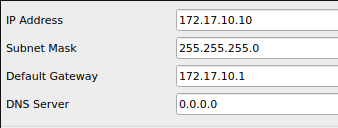
\includegraphics[width=.45\linewidth]{Figures/2020-03-19-195606_338x128_scrot.png}}\hfill
\subfloat[PC3 IP Configuration]{\label{IPC15PC3}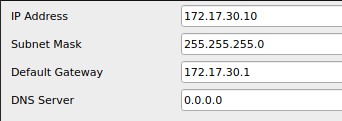
\includegraphics[width=.45\linewidth]{Figures/2020-03-19-195649_342x121_scrot.png}}\par 
\caption{IP configuration of the PCs on the network}\label{IPC15}
\end{figure}

\noindent\mysubsection{2}{Configuring the Switch and Router}\\
I then, configured the Switch and router according to the handout.

\begin{figure}[!hbt]\centering
\subfloat[show ip int brief on S1]{\label{Config15S1}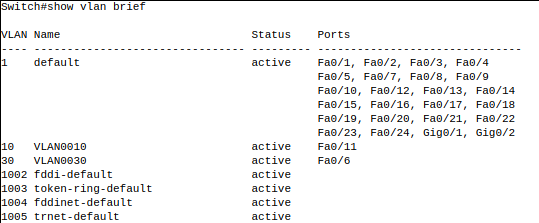
\includegraphics[width=.45\linewidth]{Figures/2020-03-19-200352_539x223_scrot.png}}\hfill
\subfloat[show vlan brief on R1]{\label{Config15R1}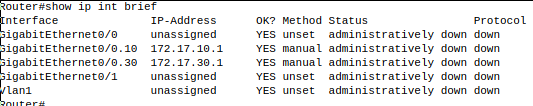
\includegraphics[width=.45\linewidth]{Figures/2020-03-19-200637_533x106_scrot.png}}\par 
\subfloat[show vlan brief on S1 after trunk config]{\label{Config15S2}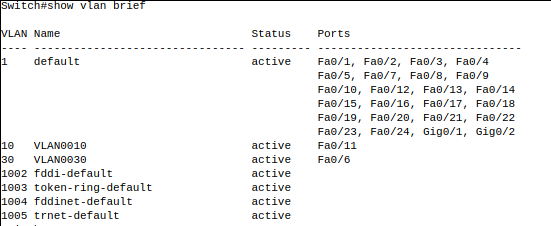
\includegraphics[width=.45\linewidth]{Figures/2020-03-19-200812_551x226_scrot.png}}
\caption{Switch and Router configuration}\label{Config15}
\end{figure}

\clearpage

\noindent\mysubsection{3}{Verifying the Network}\\
Successfully able to ping PC3 from PC1.

\begin{figure}[!hbt]\centering
\subfloat[Pinging PC3 from PC1]{\label{success15ping}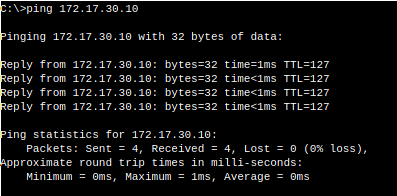
\includegraphics[width=.45\linewidth]{Figures/2020-03-08-191601_397x196_scrot.png}}\hfill
\subfloat[Successful Network Configuration]{\label{success15net}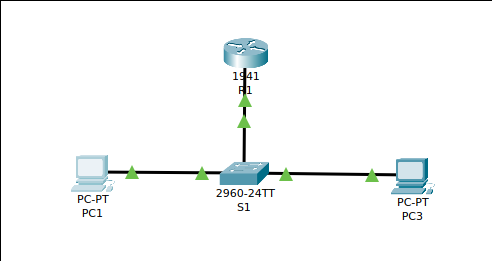
\includegraphics[width=.45\linewidth]{Figures/2020-03-08-191611_492x261_scrot.png}}\par
\caption{Successful network setup}\label{success15}
\end{figure}








%===================================

\end{document}
